\documentclass[12pt,hyperref={pdfpagelabels=false},notes=show]{beamer}

\usetheme[]{FFF}

% Bugfix for pdfpagelables=false
\providecommand\thispdfpagelabel[1]{}

% Standard packages

\usepackage[english,ngerman]{babel}
\usepackage[utf8]{inputenc}
\usepackage{times}

% Setup TikZ

\usepackage{tikz}
\usetikzlibrary{arrows}
\tikzstyle{block}=[draw opacity=0.7,line width=1.4cm]

% Text \us
\usepackage{textcomp}
\usepackage{mathcomp}

% Textpos
\usepackage[absolute,overlay]{textpos}
\setlength{\TPHorizModule}{\paperwidth}
\setlength{\TPVertModule}{\paperheight}

% Blitz-Symbol
\usepackage{stmaryrd}

% Tabellen
\usepackage{multirow}
\usepackage{array}
\usepackage{colortbl}
\definecolor{lightblue}{rgb}{ 0.55, 0.55, 1.00}
\definecolor{lightred}{rgb}{  1.00, 0.35, 0.35}
\definecolor{lightgreen}{rgb}{0.50, 1.00, 0.50}
\newcommand{\ccg}{\cellcolor{lightgreen}}
\newcommand{\ccr}{\cellcolor{lightred}}
\newcommand{\ccb}{\cellcolor{lightblue}}

% Listings
\usepackage{listings}

\setlength{\parindent}{0cm}

% Stroke
\usepackage{ulem}

% vc
\input{vc.tex}

%%%%%%%%%%%%%%%%%%%%%% /LAYOUT %%%%%%%%%%%%%%%%%%%%%%%%%%%%


% Author, Title, etc.

\title{Die L3 Transition von Freifunk Franken}

\subtitle{KNF-Kongress 2015}

\author[Tim Niemeyer]{Tim Niemeyer {\tiny \textless{}tim@freifunk-franken.de\textgreater{}}\texorpdfstring{\tiny \\\\
                        https://github.com/RedDog99/vortrag-knf.git\newline
                        \VCRevisionMod}{}}

\date[22.11.2015]{22.11.2015}

\newcommand{\zb}{z.\,B.\@}
\newcommand{\us}{~\textmu{}s}
\newcommand{\uv}{~\textmu{}V}
\newcommand{\ms}{~ms}

\begin{document}

\usebackgroundtemplate{
\includegraphics[height=\paperheight,width=\paperwidth]{slides_background_title}}

\beamertemplatenavigationsymbolsempty
\begin{frame}[plain,squeeze]
	\maketitle
\end{frame}\addtocounter{framenumber}{-1}

\usebackgroundtemplate{
\includegraphics[height=\paperheight,width=\paperwidth]{slides_background}}

\begin{frame}{Inhalt}
    \hspace{0.1\textwidth}
    \parbox[c][0.8\textheight][s]{0.8\textwidth}{
        \tableofcontents
    }
\end{frame}

%%%%%%%%%%%%%%%%%%%%%% CONTENT %%%%%%%%%%%%%%%%%%%%%%%%%%%%

\section{Einleitung}

\begin{frame}{Einleitung}
    \begin{itemize}
        \item Freifunk Franken ist lokaler Ableger der Freifunk-Bewegung (freifunk.net)
        \item Nicht-kommerzielle Initiative für freie Funknetzwerke\\
        \begin{itemize}
            \item[$\rightarrow$] Bürger investieren in Eigenregie Zeit, Geld und Enthusiasmus
        \end{itemize}
        \item Nicht nur \glqq{}kostenloses Internet\grqq $\Rightarrow$ \glqq{}freies Netzwerken\grqq\\
        \begin{itemize}
            \item Lokal intressante Dienste zur Verfügung stellen (Webcams)
            \item Text, Musik und Filme über das interne Freifunk-Netz übertragen
            \item Über lokale Dienste Chatten oder Telefonieren
        \end{itemize}
    \end{itemize}
\end{frame}

\begin{frame}{Wie es funktioniert}
    \begin{itemize}
        \item Freifunker stellen WLAN-Router für sich selbst und den Datentransfer der anderen Teilnehmer zur Verfügung
        \begin{itemize}
            \item ggf. mit Anschluss an das www (für VPN)
        \end{itemize}
        \item Benachbarte Router verbinden sich und spannen ein sogenanntes Mesh-Netzwerk auf
        \item Nicht benachbarte Router verbinden sich mittels VPN-Tunnel zum Freifunk
        \item Jegliche Verbindung ins www wird hierüber umgeleitet, um Risiken der Störerhaftung zu entgehen
    \end{itemize}
\end{frame}

\begin{frame}{Was braucht man?}
    \begin{itemize}
        \item Ein günstiger, unterstützter Router (ab ca. 17€)
        \item Eine spezielle Firmware
        \item Die Zustimmung zum \glqq{}Pico-Peering Agreement\grqq
        \begin{itemize}
            \item Regelwerk, das grundsätzliche Eigenschaften eines Freifunk-Netzwerkes sichert
            \begin{enumerate}
                \item Freier Transit
                \item Offene Kommunikation
                \item Keine Garantie (Haftungsausschluss)
                \item Nutzungsbestimmungen
                \item Lokale (individuelle) Zusätze
            \end{enumerate}
            \item Die Freifunk Firmware implementiert diese Grundsätze standardmäßig
        \end{itemize}
    \end{itemize}
\end{frame}

\begin{frame}{Ein typisches Freifunk Netz}
    todo Bild eines typischen Freifunk Netzes
\end{frame}

\section{Mesh Router}

\begin{frame}{Software}
    \begin{itemize}
        \item OpenWRT mit
        \item Batman-Adv
        \item Fastd
        \item Nodewatcher
        \item Fastdstart
        \item .. weiteren kleineren Tools
        \item .. configs und scripten
    \end{itemize}
\end{frame}

\begin{frame}{von aussen}
    \begin{itemize}
        \item Client-Ports \& Infrastructure Funknetz:
            Wie ein großer Switch
        \item Batman-Ports \& Ad-Hoc Funknetz:
            Mesh-Netz
        \item WAN-Ports:
            VPN Netz
    \end{itemize}
    \center{
        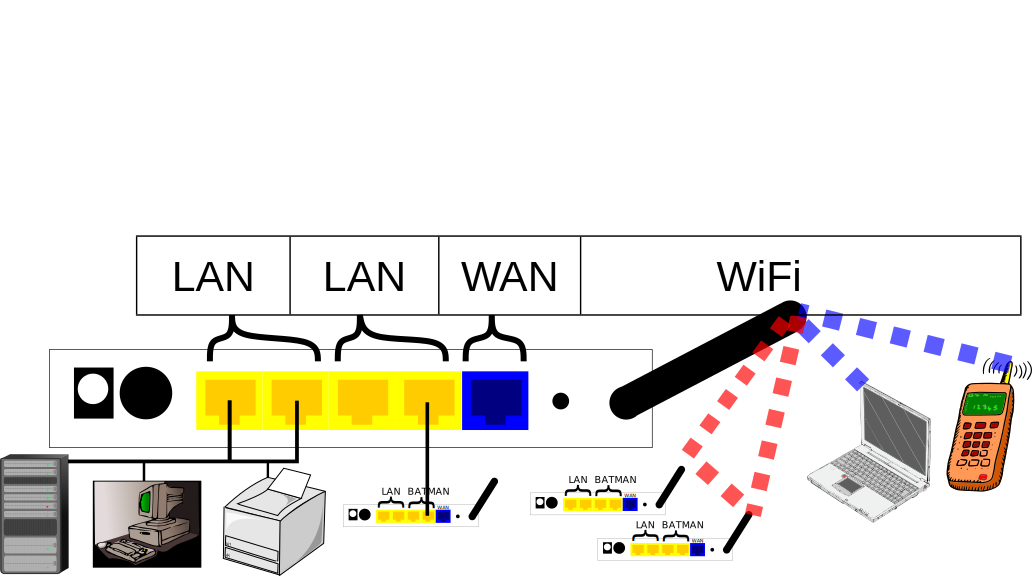
\includegraphics[width=0.75\textwidth]{img/svg/anschluesse.pdf}
    }
\end{frame}

\begin{frame}{von innen}
    \renewcommand{\arraystretch}{1.5}
    \begin{tabular}{|c|c|c|c|c|c|c|} \hline
         \multicolumn{7}{|c|}{Bridge} \\ \hline
         \multirow{2}{*}{Managed} &
         \multicolumn{4}{c|}{B.A.T.M.A.N} &
         \multicolumn{2}{c|}{\multirow{2}{*}{Client-VLan}} \\ \cline{2-5}
         & Ad-Hoc & VPN & \multicolumn{2}{c|}{Node-VLan} & \multicolumn{2}{c|}{} \\ \hline
         \multicolumn{2}{|c|}{Wifi} & WAN & LAN1 & LAN2 &
         LAN3 & LAN4 \\ \hline
    \end{tabular}

    \begin{itemize}
        \item Jeder Knoten ist wie ein großer Switch
    \end{itemize}
\end{frame}


\include{firmware}
\section{VPN}

%Wie die Wireless Mesh Verbindungen zustande kommen geht aus dem
%Aufbau der Firmware bereits hervor. Wie jedoch die Knoten
%untereinander verbunden werden, soll der Vortrag in einem weiteren
%Abschnitt über das verwendete VPN zeigen. Dazu gehört auch die
%Aufteilung in Subnetze und die Verbindung der Gateways
%untereinander.

\begin{frame}{Allgemeines}
    \begin{itemize}
        \item Verwendetes VPN: fastd
        \item Layer-II Netz
        \item Wir nutzen keine Verschlüsselung (! :-O)
    \end{itemize}
    \begin{block}{fastd}
        % todo: was ist fastd ?
        There are no server and client roles defined by the
        protocol, this is just defined by the usage.
        \begin{itemize}
            \item Only one instance of the daemon is needed on each
                host to create a full mesh
            \item If no full mesh is established, a routing protocol
                is necessary to enable hosts that are not connected
                directly to reach each other
        \end{itemize}
    \end{block}
\end{frame}

\begin{frame}{Allgemeines}
    \begin{itemize}
        \item fastd Integration durch
        \begin{itemize}
            \item fastdstart.sh auf der Client-Seite
                \footnote{bsp/default/root\_file\_system/etc/fastdstart.sh.tpl}
            \item \$project\_\$hood\_fastd.sh auf der Server-Seite
                \footnote{auf den Gateways (!) Todo: befreien!}
            \item VPN-KeyXchange als Schlüsseltausch
                \footnote{\url{https://github.com/FreifunkFranken/VPNkeyXchange}}
        \end{itemize}
        \item Aufteilung in ,,hood''s:
        \begin{itemize}
            \item Stellt ein Layer-II Netz dar
            \item Ein Gateway kann mehrere Layer-II Netze bedienen
        \end{itemize}
    \end{itemize}
\end{frame}

\begin{frame}{Freifunk Hoods}
    \includegraphics[width=\textwidth]{img/svg/freifunk_konzepte.pdf}

    Unser Freifunknetz ist in mehrere Layer-2 Inseln, die per Layer-3 miteinander verbunden sind,
    aufgeteilt. Die Hoods A und B in diesem Beispiel sind über unser VPN jeweise mit einem Router im
    Internet verbunden. Hood C hat einen lokalen Router, der direkt am LAN-Port hängt.
\end{frame}

\begin{frame}{\alt<1>{fastdstart.sh}{\$project\_\$hood\_fastd.sh}}
    \begin{itemize}
        \item \only<1>{Testet Internet-Connectivität}
        \item Legt fastd Konfiguration
            /etc/fastd/\$project\only<2>{.\$hood}/ \only<1>{im tmpfs} an:
            \footnote{\$project ist bei uns immer ,,fff''.}
            \begin{itemize}
                \item \$project.conf
                \item up.sh
                \item down.sh
                \item peers/
            \end{itemize}
        \item Erzeugt Pub/Priv-Keypaar
        \item Startet fastd
        \item Meldet sich beim VPN-KeyXchange an
        \item Lädt Liste mit Peers
        \item Refresht fastd
        \item \only<2>{Löscht verwaiste Peers}
    \end{itemize}
\end{frame}

\begin{frame}{VPN-KeyXchange}
    \begin{itemize}
        \item Knoten Identifizierung über MAC, alternativ über Name
        \item Jeweils pro hood:
        \begin{itemize}
            \item Clients bekommen eine Liste aller Gateways
            \item Gateways bekommen eine Liste aller Clients+Gateways
        \end{itemize}
    \end{itemize}
\end{frame}

\section{Gateway}

%Über die Gateways steht i.d.R. auch eine Internetverbindung zur
%Verfügung. Auch die Installation dieser Gateways sollen daher Teil
%des Vortrags sein.

\begin{frame}{Was macht ein Gateway?}
    \begin{itemize}
        \item VPN
        \item DHCP
        \item DNS
        \item Policy base routing
        \item Routing zu anderen Gateways
        \item Optional Routing ins Internet
    \end{itemize}
\end{frame}

\begin{frame}{Internet Traffic}
    Aufteilung von Gateways in Hood-Server und Gateways.
\end{frame}

\begin{frame}{DNS}
    \begin{itemize}
        \item Bind
        \item fff.community
    \end{itemize}
\end{frame}


\section{Netmon}

%Ein spezieller Dienst im Freifunk Franken Netz ist das
%Network-Monitoring, kurz Netmon. Netmon selbst soll nicht Teil des
%Vortrags sein, wohl aber die Verbindung zwischen Netmon und den
%Knoten. Dazu zählt zum Beispiel das Handling der Hostnames und das
%Einsammeln der Statusdaten.

\begin{frame}{Netmon}
    \begin{itemize}
        \item Nodewatcher
        \begin{itemize}
            \item Generiert Status-Daten
            \item XML
            \item alle 5 Minuten
        \end{itemize}
        \item Configurator
        \begin{itemize}
            \item Verknüpft Netmon und Knoten
        \end{itemize}
        \item Crawler
        \begin{itemize}
            \item Sammelt Status-Daten
            \item Download über http Schnittstelle der Knoten
            \item Alles über Link-Local
        \end{itemize}
        \item Netmon
        \begin{itemize}
            \item Visualisiert Status-Daten
        \end{itemize}
    \end{itemize}
\end{frame}

\begin{frame}{Monitoring}
    \begin{itemize}
        \item Alfred
        \item todo Bild alfred masters auf jedem GW
    \end{itemize}
\end{frame}

%\include{aktuelles}

\section*{}
\begin{frame}{Ende}
    \begin{center}
        Vielen Dank für Eure Aufmerksamkeit	...
     \end{center}
\end{frame}\addtocounter{framenumber}{-1}
	
\section*{}
\include{reserve}

%%%%%%%%%%%%%%%%%%%%%% /CONTENT %%%%%%%%%%%%%%%%%%%%%%%%%%%%

\end{document}
